\pagestyle{fancy}
\setlength{\headheight}{16pt}
\fancyhead{} % clear all header fields
\fancyhead[L]{\textbf{CEE 576 Homework 3}}
\fancyhead[C]{Songyuan Cui}
\fancyhead[R]{\textbf{Fall 2024}}
\fancyfoot{} % clear all footer fields
\fancyfoot[C]{\thepage}

\newcommand{\Fint}{\ensuremath{\bv{F}^{\textrm{int}}}}
\newcommand{\Fext}{\ensuremath{\bv{F}^{\textrm{ext}}}}

\noindent \emph{Disclaimer}. All computer programs in this assignment are implemented in \matlab~and can be found at \url{https://github.com/sy-cui/CSE552-FA2024/tree/main/homework/hw3}. 
\emph{A \texttt{README.md} file is provided in the same directory for reference}. 
The codes are tested in \matlab~version 2024a. 
However, latest \matlab~features are intentionally avoided to maximize backward-compatibility, so the code should work out-of-the-box with most \matlab~versions. 
The directory is self-containing and does not dependent on external programs or packages. 
However, please make sure to copy \emph{the entire directory} as there are functions defined in individual files that are used by other files. 

\section{Show that small strain ``epsilon'' is not zero for the rigid body motion}
The infinitesimal (small) strain $\bt{\epsilon}$ is defined as 
\begin{equation}
    \epsilon_{ij} = \frac{1}{2}\left(\frac{\partial u_i}{\partial X_j} + \frac{\partial u_j}{\partial X_i}\right) \equiv \frac{1}{2}\left(\textrm{GRAD} \bv{u} + \textrm{GRAD} \bv{u}^T\right)
\end{equation}
where $\bv{u} = \bv{\varphi}(\bv{X}, t) - \bv{X}$ is the displacement field.
A rigid-body motion consists of a rotation ($\bt{Q}(t)$) and a translation ($\bv{c}(t)$) such that 
\begin{equation}\label{eqn:hw3_p1_rigid}
    \bv{x} = \bv{\varphi}(\bv{X}, t) = \bt{Q}(t) \bv{X} + \bv{c}(t), ~~~~ \bt{Q}(t)\in SO(3).
\end{equation}
It then follows that $\textrm{GRAD}\bv{u} = \bt{Q}(t) - \bt{I}$. 
The infinitesimal strain after the rigid-body motion reads
\begin{equation}
    \bv{\epsilon} \equiv \frac{1}{2}(\bt{Q} + \bt{Q}^T - 2\bt{I})
\end{equation}
which is \emph{in general non-zero} unless $\bt{Q} = \bt{I}$ which implies pure translation.
Therefore, the infinitesimal strain tensor $\bv{\epsilon}$ does not remain zero after rigid-body motion and is hence not an appropriate strain measure for geometric nonlinearities. Q.E.D.

\section{Derive the material time derivative for a scalar and a tensor field}
\begin{enumerate}[(a)]
\item {
    Given a scalar field $f(\bv{x}, t) = F(\bv{X}, t)$, the material time derivative is 
    \begin{equation}
        \frac{\partial F}{\partial t} \equiv \frac{Df}{Dt} = \frac{\partial f}{\partial t} + \frac{\partial f}{\partial x_i}\frac{\partial \varphi_i(\bv{X}, t)}{\partial t} = \frac{\partial f}{\partial t} + v_i \frac{\partial f}{\partial x_i},
    \end{equation}
    where the Eulerian velocity field is defined as 
    \begin{equation}
        v_i(\bt{x}, t) = V_i(\bt{X}, t) :=  \frac{\partial \varphi_i(\bt{X}, t)}{\partial t}.
    \end{equation}
}
\item {
    Given a tensor field $\sigma_{ij}(\bv{x}, t) = \Sigma_{ij}(\bv{X}, t)$, the material time derivative is 
    \begin{equation}
        \frac{\partial \Sigma_{ij}}{\partial t} \equiv \frac{D\sigma_{ij}}{Dt} = \frac{\partial \sigma_{ij}}{\partial t} + \frac{\partial \sigma_{ij}}{\partial x_k}\frac{\partial \varphi_k(\bv{X}, t)}{\partial t} = \frac{\partial \sigma_{ij}}{\partial t} + v_k \frac{\partial \sigma_{ij}}{\partial x_k},
    \end{equation}
    Typically, the material derivatives can be written in the form 
    \begin{equation}
        \frac{D(\cdot)}{Dt} = \frac{\partial (\cdot)}{\partial t} + \bv{v} \cdot \del(\cdot)
    \end{equation}
    which applies to scalar, vector, and tensor fields. 
}
\end{enumerate}

\section{Show that Green's strain tensor is invariant under rigid-body motion (when it is zero)}
The Green(-Lagrange) strain tensor is defined as 
\begin{equation}\label{eqn:hw3_p3_green}
    \bt{E}:= \frac{1}{2}(\bt{F}^T \bt{F} - \bt{I}) = \frac{1}{2}(\textrm{GRAD}\bv{u} + \textrm{GRAD}\bv{u}^T + \textrm{GRAD}\bv{u}~\textrm{GRAD}\bv{u}^T).
\end{equation}
We again consider the rigid-body motion \cref{eqn:hw3_p1_rigid} which leads to $\textrm{GRAD}\bv{u} = \bt{Q}(t) - \bt{I}$. 
Substitution into \cref{eqn:hw3_p3_green} leads to 
\begin{equation}
    \bt{E} = \frac{1}{2}\left[\bt{Q} + \bt{Q} - 2\bt{I} + \left(\bt{I} - \bt{Q} - \bt{Q}^T + \bt{Q}\bt{Q}^T\right)\right] = \bt{0}
\end{equation}
where we have used the orthogonality of the rotation matrix $\bt{Q}\bt{Q}^T = \bt{Q}^T \bt{Q} = \bt{I}$.

\section{Arc-length method}
Given a reference load vector $\Fext$ and a set of converged solution $\bv{u}_n$ and $\lambda_n$ such that $\Fint(\bv{u}_n) = \lambda_n \Fext$, the goal of the arc-length method is to solve the following system of nonlinear equations
\begin{subequations}
\begin{equation}\label{eqn:hw3_gov}
    \Fint(u) = \lambda \Fext
\end{equation}
\begin{equation}\label{eqn:hw3_gov_arc}
    f(\bv{u} - \bv{u}_n, \lambda - \lambda_n) = f(\delta \bv{u}, \delta\lambda) = \delta a
\end{equation}
\end{subequations}
where $\delta a$ is a prescribed step-size parameter and $f(\delta \bv{u}, \delta \lambda)$ is an ellipsoidal arc-length function chosen as 
\begin{equation}
    f(\delta \bv{u}, \delta \lambda) := \left(c \delta \bv{u}^T \textrm{diag}(\bt{K}_0) \delta \bv{u} + b \delta\lambda^2\right)
\end{equation}
where $\bt{K}_0$ is the tangent matrix at $t = 0$, and $b$ and $c$ are pre-defined constants with 
\begin{equation}\label{eqn:hw3_c}
    c := \frac{1 - b}{\bv{q}_0^T {\textrm{diag}(\bt{K}_0)} \bv{q}_0}, ~~~~ \bv{q}_0 := \bt{K}_0^{-1} \Fext
\end{equation}
It is convenient to define the displacement-like vector $\bv{q} := \bt{K}^{-1} \Fext$ which should be differentiated from $\bv{q}_0$ defined above.
To solve the nonlinear system \cref{eqn:hw3_gov,eqn:hw3_gov_arc}, we employ the Newton-like iteration technique 
\begin{equation}\label{eqn:hw3_step_block}
    \underbrace{\begin{bmatrix}
        \bt{K}^{(i)} & -\Fext \\ {\left(\frac{\partial f}{\partial \delta \bv{u}}\right)}_i^{T} & {\left(\frac{\partial f}{\partial \delta \lambda}\right)}_i
    \end{bmatrix}}_{\mathbb{A}^{(i)}}
    \begin{bmatrix}
        \Delta \bv{u}^{(i)} \\ \Delta \lambda^{(i)}
    \end{bmatrix}
    = \begin{bmatrix}
        \lambda^{(i)} \Fext - \Fint(\bv{u}^{(i)}) \\ \delta a - f(\delta \bv{u}^{(i)}, \delta \lambda^{(i)})
    \end{bmatrix}
\end{equation}
where one has the freedom to choose the $\bv{u}$ and $\lambda$ with respect to which $\mathbb{A}^{(i)}$ is computed. 
In this exercise, we use (MNR for $\bt{K}$, NR for $f$)
\begin{equation}
    \bt{K}^{(i)} = \frac{d\Fint}{d\bv{u}}\Bigg|_{\bv{u} = \bv{u}_n}, ~~~~ 
    {\left(\frac{\partial f}{\partial \delta \bv{u}}\right)}_i = {\left(\frac{\partial f}{\partial \delta \bv{u}}\right)}\Bigg|_{\delta \bv{u} = \delta \bv{u}^{(i)}}, ~~~~
    {\left(\frac{\partial f}{\partial \delta \lambda}\right)}_i = {\left(\frac{\partial f}{\partial \delta \lambda}\right)}\Bigg|_{\delta \lambda = \delta \lambda^{(i)}}
\end{equation}
Note that \cref{eqn:hw3_step_block} can be solved in a staggered manner. 
Specifically, consider the following Schur's complement form of a symbolic system of equations
\begin{equation}
\begin{aligned}
    && \begin{bmatrix}
        \bt{A} & \bt{B} \\ \bt{C} & \bt{D}
    \end{bmatrix} 
    \begin{bmatrix}
        \bv{x} \\ \bv{y}
    \end{bmatrix} &= \begin{bmatrix}
        \bv{e} \\ \bv{f}
    \end{bmatrix} \\ \Rightarrow && 
    \begin{bmatrix}
        \bt{I} & \bt{0} \\ -\bt{C}\bt{A}^{-1} & \bt{I}
    \end{bmatrix} 
    \begin{bmatrix}
        \bt{A} & \bt{B} \\ \bt{C} & \bt{D}
    \end{bmatrix} 
    \begin{bmatrix}
        \bv{x} \\ \bv{y}
    \end{bmatrix} &= 
    \begin{bmatrix}
        \bt{I} & \bt{0} \\ -\bt{C}\bt{A}^{-1} & \bt{I}
    \end{bmatrix} 
    \begin{bmatrix}
        \bv{e} \\ \bv{f}
    \end{bmatrix} \\ \Rightarrow && 
    \begin{bmatrix}
        \bt{A} & \bt{B} \\ \bt{0} & \bt{D - \bt{C}\bt{A}^{-1}\bt{B}}
    \end{bmatrix} 
    \begin{bmatrix}
        \bv{x} \\ \bv{y}
    \end{bmatrix} &= 
    \begin{bmatrix}
        \bv{e} \\ \bv{f} - \bt{C}\bt{A}^{-1}\bv{e}
    \end{bmatrix}
\end{aligned}
\end{equation}
which can then be solved using back-substitution. 
Define 
\begin{equation}
    \bv{R}^{(i)} = \lambda^{(i)} \Fext - \Fint(\bv{u}^{(i)}), ~~~~ \bv{v}^{(i)} = {\bt{K}^{(i)}}^{-1} \bv{R}^{(i)}
\end{equation}
then
\begin{subequations}
\begin{equation}\label{eqn:hw3_Du}
    \Delta \lambda^{(i)} = \frac{\delta a - f(\delta \bv{u}^{(i)}, \delta \lambda^{(i)}) - {\left(\frac{\partial f}{\partial \delta \bv{u}}\right)}_i^T \bv{v}^{(i)}}{{\left(\frac{\partial f}{\partial \delta \lambda}\right)}_i + {\left(\frac{\partial f}{\partial \delta \bv{u}}\right)}_i^T \bv{q}}
\end{equation}
\begin{equation}\label{eqn:hw3_Dl}
    \Delta \bv{u}^{(i)} = \Delta \lambda^{(i)} \bv{q} + \bv{v}^{(i)}
\end{equation}     
\end{subequations} 
with 
\begin{equation}\label{eqn:hw3_arc_grad}
    {\left(\frac{\partial f}{\partial \delta \bv{u}}\right)}_i = \frac{c\cdot \textrm{diag}(\bt{K}_0)\delta \lambda^{(i)}}{f(\delta\bv{u}^{(i)}, \delta \lambda^{(i)})}, ~~~~{\left(\frac{\partial f}{\partial \delta \lambda}\right)}_i = \frac{b\delta \lambda^{(i)}}{f(\delta\bv{u}^{(i)}, \delta \lambda^{(i)})}
\end{equation}
Finally, one needs an initial guess for $\delta \lambda^{(0)}$ and $\delta \bv{u}^{(0)}$ as it is evident that setting them to zero leads to zero gradient, rendering $\mathbb{A}$ singular.
\emph{It should be noted that the initial guess is by no means unique and any choice that leads to convergence is reasonable.} 
Here, we choose $|\delta \lambda^{(0)}| = \delta a$ with the sign dependent upon the change in consistent tangent ($\det(\bt{K})$). 
If $\det(\bt{K})$ change sign through zero (zero-slope limiting point), then $\delta \lambda^{(0)}$ change sign with respect to the previously used $\delta \lambda^{(0)}$. 
$\delta \bv{u}^{(0)}$ is set to be $\pm \delta a \bv{q}_0$, whose sign can change due to infinite-slope limiting point (not present in this exercise).
\emph{The general algorithm is shown in} \cref{alg:hw3_alm}, \emph{which should be sufficiently detailed and hence the flow chart is omitted}. 

\begin{algorithm}[!ht]
\caption{Arc-length method using Modified-Newton-Raphson iterations}
\begin{algorithmic}[1]\label{alg:hw3_alm}
    \setlength{\lineskip}{4pt}
    \Require{Nonlinear function $\Fint(\bv{u})$, reference external load $\Fext$, arc-length function $f(\delta \bv{u}, \delta \lambda)$, arc-length parameter $\delta a$, initial displacement $\bv{u}_0$, initial load parameter $\lambda_0$, step-control parameter $b$, tolerance for relative residual $\epsilon_n$, tolerance for arc-length $\epsilon_a$}
    \Ensure{Solution $\bv{u}_n$, $\lambda_n \Fext$ along the load-displacement curve}

    \item[] % line-break

    \State{$\bt{K}_0 \gets \partial_{\bv{u}} \Fint (\bv{u}_0)$ }
    \Comment{Reference tangent matrix}

    \State{$\bv{q}_0 \gets \bt{K}_0^{-1} \Fext$}

    \State{Compute $c$ using \cref{eqn:hw3_c}}

    \item[] % line-break

    \If{$\det(\bt{K}_0) > 0$}
    \Comment{Determine initial load parameter change}
    \State{$\delta \lambda_0^{(0)} \gets \delta a$}
    \Else{}
    \State{$\delta \lambda_0^{(0)} \gets -\delta a$}
    \EndIf{}

    \item[] % line-break

    \For{$n = 1, 2, \ldots, N$}
    \Comment{For every load step}

    \State{$\bt{K}_n \gets \partial_{\bv{u}} \Fint (\bv{u}_n)$}
    \Comment{Consistent tangent matrix}

    \State{$\bv{q}_n \gets \bt{K}_n^{-1} \Fext$}

    \If{$\det(\bt{K}_n)\cdot \det(\bt{K}_{n-1}) > 0$}
    \Comment{Creat an initial guess}
    \State{$\delta \lambda_n^{(0)} \gets \delta \lambda_{n-1}^{(0)}$}
    \Else{}
    \State{$\delta \lambda_n^{(0)} \gets -\delta \lambda_{n-1}^{(0)}$}
    \EndIf{}

    \State{$\delta \bv{u}^{(0)} \gets \delta a \bv{q}_n$}

    \item[] % line-break

    \State{$\bv{u}_n^{(0)} \gets \bv{u}_{n-1} + \delta \bv{u}_n^{(0)}$}
    \Comment{Initial guess of displacement}

    \State{$\lambda_n^{(0)} \gets \lambda_{n-1} + \delta \lambda_n^{(0)}$}
    \Comment{Initial guess of load parameter}

    \State{$\bv{R}_n^{(0)} \gets \lambda_n^{(0)}\Fext - \Fint(\bv{u}_n^{(0)})$}
    \Comment{Initial main residual}

    \State{$\bv{r}_n^{(0)} \gets \delta a - f(\delta \bv{u}_n^{(0)}, \delta \lambda_n^{(0)})$}
    \Comment{Initial arc-length residual}

    \State{$\bv{v}_n^{(0)} \gets \bt{K}_n^{-1} \bv{R}_n^{(0)}$}

    \item[] % line-break
 
    \State{$k \gets 1$}

    \While{$\| R_n^{(k)}\|_{\bt{K}_n^{-1}} / \| R_n^{(0)}\|_{\bt{K}_n^{-1}} > \epsilon_n$ or $| r_n^{(k)}| / \delta a > \epsilon_a$}
    \Comment{Modified Newton-Raphson iterations}
        
        \State{Compute $\partial_{\delta \bv{u}} f(\delta \bv{u}^{(k)}, \lambda_n^{(k)})$, $\partial_{\delta \lambda} f(\delta \bv{u}_n^{(k)}, \lambda_n^{(k)})$ using \cref{eqn:hw3_arc_grad}}

        \State{Compute $\Delta \bv{u}_n^{(k)}$, $\Delta \lambda_n^{(k)}$ using \cref{eqn:hw3_Du,eqn:hw3_Dl}}

        \item[] % line-break

        \State{
            $\bv{u}_n^{(k+1)} \gets \bv{u}_n^{(k)} + \Delta \bv{u}_n^{(k)}$, 
            $\delta \bv{u}_n^{(k+1)} \gets \delta \bv{u}_n^{(k)} + \Delta \bv{u}_n^{(k)}$}
        \Comment{Update displacement}

        \State{
            $\lambda_n^{(k+1)} \gets \lambda_n^{(k)} + \Delta \lambda_n^{(k)}$, 
            $\delta \lambda_n^{(k+1)} \gets \delta \lambda_n^{(k)} + \Delta \lambda_n^{(k)}$}
        \Comment{Update load parameter}

        \item[] % line-break

        \State{$\bv{R}_n^{(k)} \gets \lambda_n^{(k)}\Fext - \Fint(\bv{u}_n^{(k)})$}
        \Comment{Update main residual}

        \State{$\bv{r}_n^{(k)} \gets \delta a - f(\delta \bv{u}_n^{(k)}, \delta \lambda_n^{(k)})$}
        \Comment{Update arc-length residual}

        \State{$\bv{v}_n^{(k)} \gets \bt{K}_n^{-1} \bv{R}_n^{(k)}$}

        \State{$k \gets k + 1$}
    \EndWhile{}

    \item[] % line-break

    \State{$\bv{u}_n \gets \bv{u}_n^{(k)}$}
    \Comment{Converged displacement of the $n$-th load step}

    \State{$\lambda_n \gets \lambda_n^{(k)}$}
    \Comment{Converged load parameter of the $n$-th load step}

    \EndFor{}
\end{algorithmic}
\end{algorithm}

We demonstrate \cref{alg:hw3_alm} for the scalar nonlinear equation 
\begin{equation}
    N(u) = \left(0.19u^3 - 2.1u^2 + 5.8 u\right) e^{0.03u}
\end{equation}
A relative residual tolerance of $\epsilon_n = 10^{-12}$ and arc-length tolerance of $\epsilon_a = 10^{-5}$ are used. 
Recall that the convergence criteria here is defined as 
\begin{subequations}
    \begin{equation}\label{eqn:hw3_main_res}
        \bar{R}_n^{(k)}:= \frac{\| \bv{R}_n^{(k)}\|_{\bt{K}^{-1}}}{\| \bv{R}_n^{(0)}\|_{\bt{K}^{-1}}} = \frac{\sqrt{{\bv{R}_n^{(k)}}^T \bv{K}_n^{-1} \bv{R}_n^{(k)}}}{\sqrt{{\bv{R}_n^{(0)}}^T \bv{K}_n^{-1} \bv{R}_n^{(0)}}} \leq \epsilon_n,
    \end{equation}
    \begin{equation}\label{eqn:hw3_arc_res}
        \bar{r}_n^{(k)}:= \frac{|r_n^{(k)}|}{\delta a} = \left| \frac{f(\delta \bv{u}_n^{(i)}, \delta \lambda_n^{(i)})}{\delta a} - 1\right| \leq \epsilon_a.
    \end{equation}
\end{subequations}
We aim to solve this problem using a fixed arc-step of $\delta a = 0.2$, zero initial displacement and load parameter, and two different step-control parameter $b = 0.5$ and $b = 0.7$. 
\emph{Due to the shear number of data points involved, the residual and convergence history is depicted via a semi-log plot of} \cref{eqn:hw3_main_res,eqn:hw3_arc_res} \emph{rather than tabulation}. 
Specifically, the solution and residual history for $b = 0.5$ ($\Fext = 5$, $26$ load steps) are shown in \cref{fig:hw3_b0pt5_soln,fig:hw3_b0pt5_res}, respectively, while those for $b = 0.7$ ($\Fext = 3$, $35$ load steps) are show in \cref{fig:hw3_b0pt7_soln,fig:hw3_b0pt7_res}.
A close-up snapshot of the solution for $b = 0.7$ is shown in \cref{fig:hw3_b0pt7_close}.
We note the initial step tend to overshoot beyond the elliptical boundary. 
This can potentially be improved bia the line-search technique.

\begin{figure}[!ht]
    \centering
    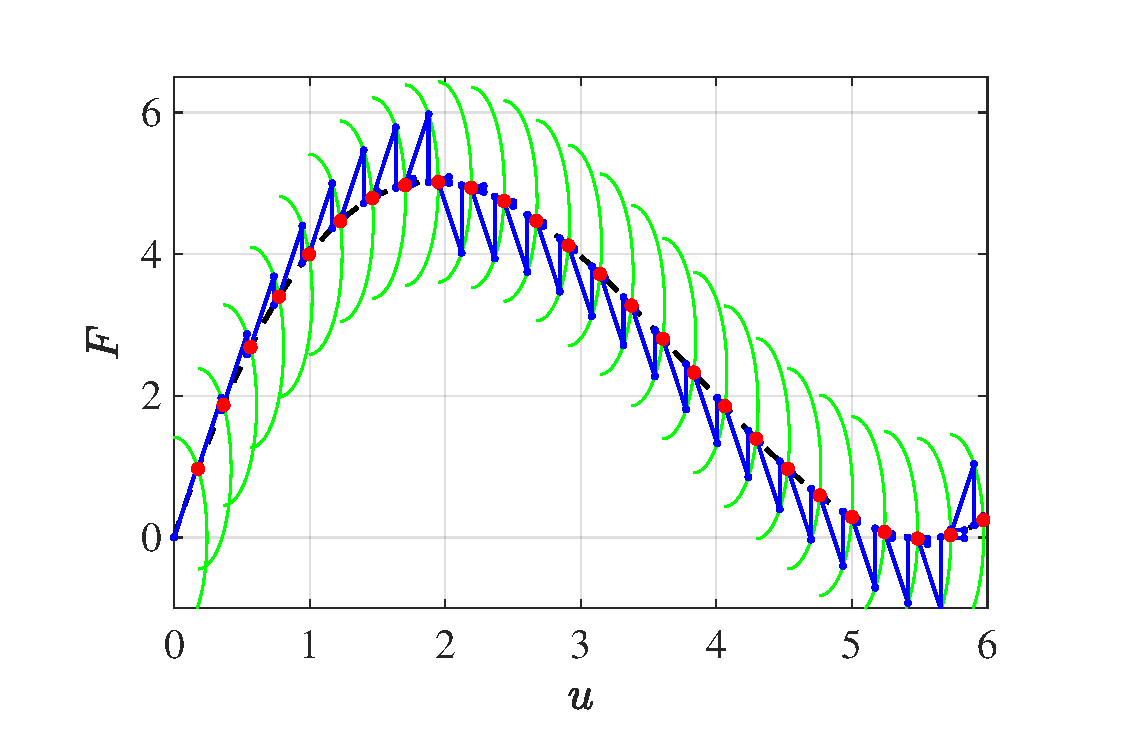
\includegraphics[width=0.7\linewidth]{homework/hw3/hw3_b0pt5_soln.pdf}
    \caption{Solution profile using the arc-length method with $b = 0.5$, $\Fext = 5$. 
    Red points denote the converged solution of each load step, and blue trajectories show the history of each iterations. 
    Green arcs represent the target boundary of the ellipsodial arc-length function.}
    \label{fig:hw3_b0pt5_soln}
\end{figure}

\begin{figure}[!ht]
    \centering
    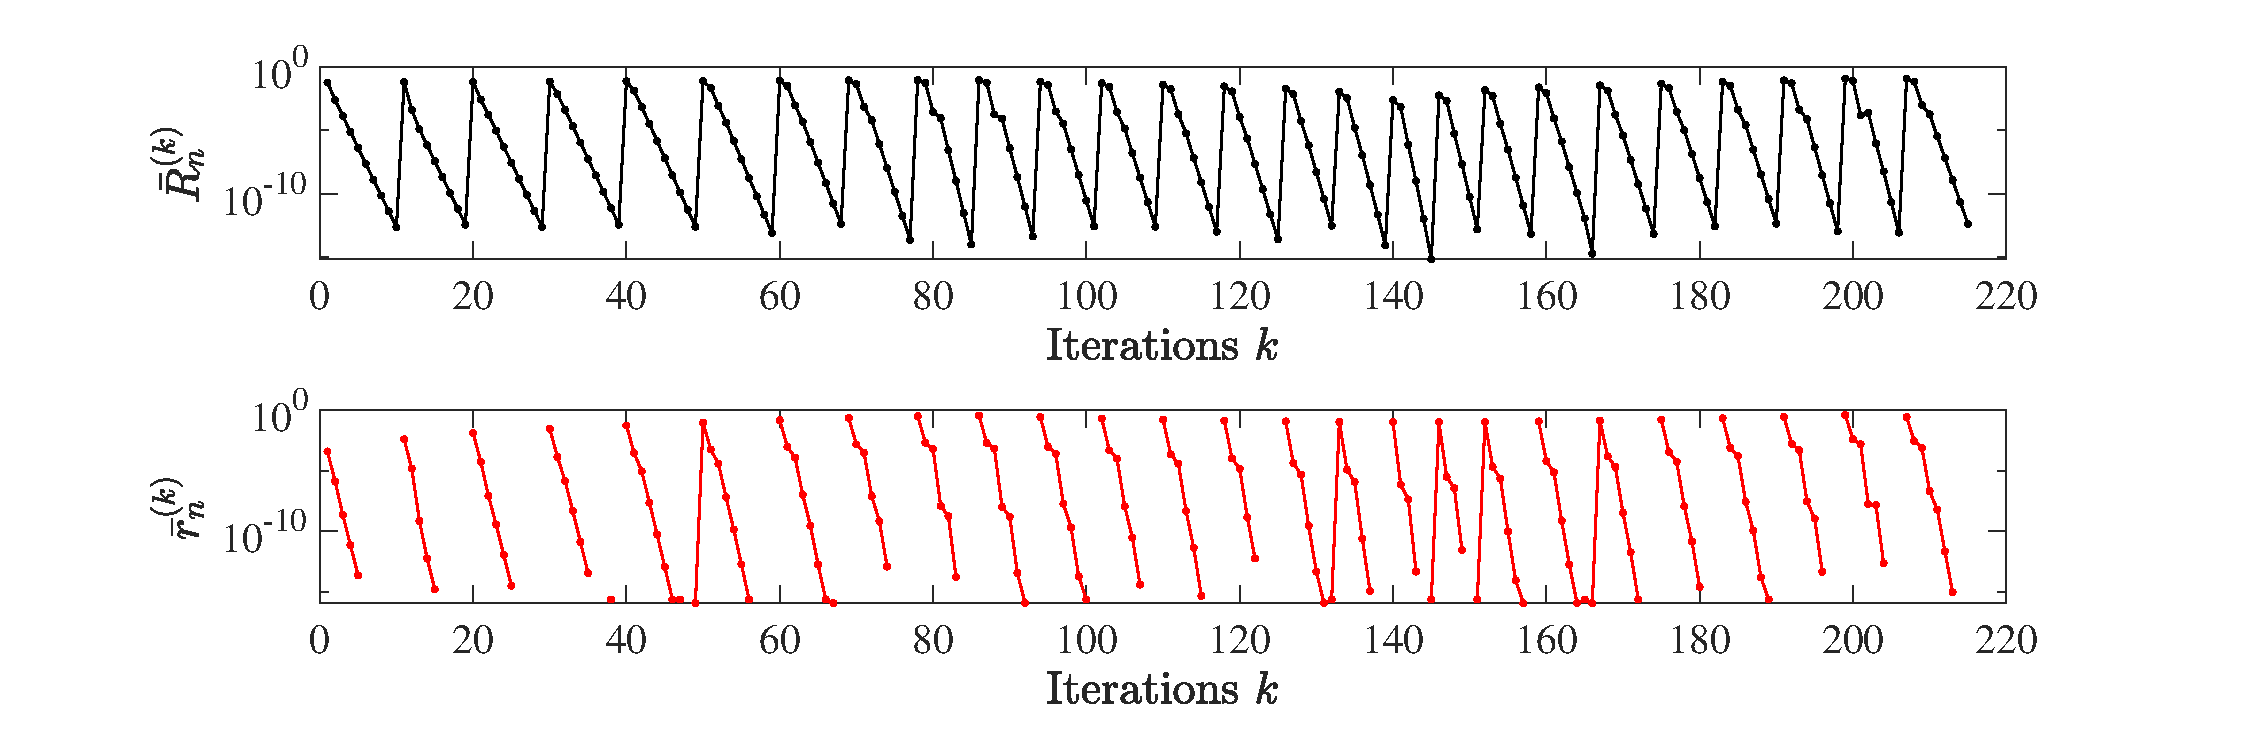
\includegraphics[width=\linewidth]{homework/hw3/hw3_b0pt5_res.pdf}
    \caption{Residual history of arc-length method with $b = 0.5$, $\Fext = 5$. 
    The upper plot shows the evolution of the main relative residual \cref{eqn:hw3_main_res} while the lower plot show that of the arc-length \cref{eqn:hw3_arc_res}.}
    \label{fig:hw3_b0pt5_res}
\end{figure}

\begin{figure}[!ht]
    \centering
    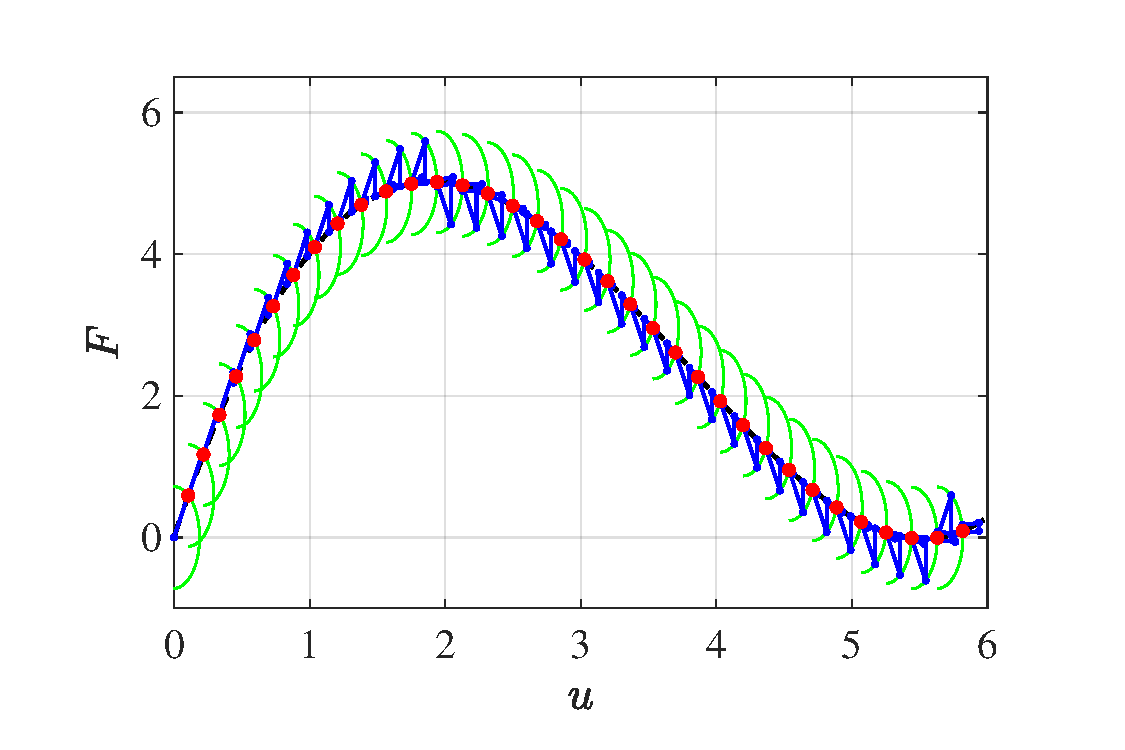
\includegraphics[width=0.7\linewidth]{homework/hw3/hw3_b0pt7_soln.pdf}
    \caption{Solution profile using the arc-length method with $b = 0.7$, $\Fext = 3$. 
    Red points denote the converged solution of each load step, and blue trajectories show the history of each iterations. 
    Green arcs represent the target boundary of the ellipsodial arc-length function.}
    \label{fig:hw3_b0pt7_soln}
\end{figure}

\begin{figure}[!ht]
    \centering
    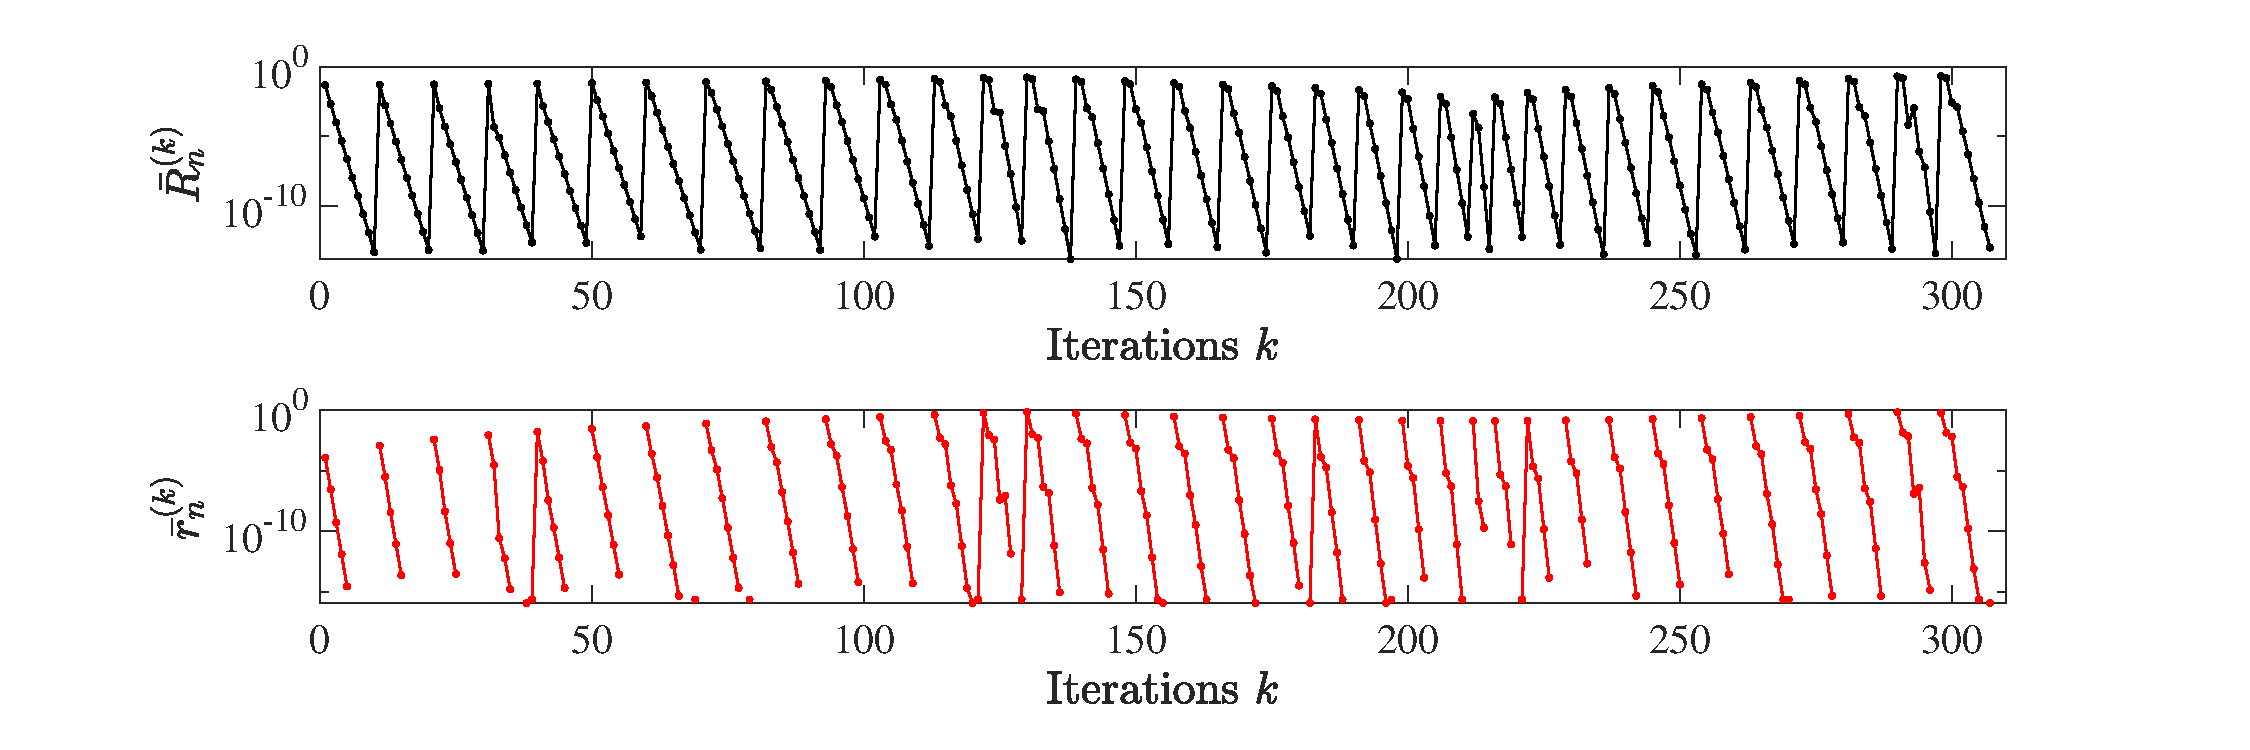
\includegraphics[width=\linewidth]{homework/hw3/hw3_b0pt7_res.pdf}
    \caption{Residual history of arc-length method with $b = 0.7$, $\Fext = 3$. 
    The upper plot shows the evolution of the main relative residual \cref{eqn:hw3_main_res} while the lower plot show that of the arc-length \cref{eqn:hw3_arc_res}.}
    \label{fig:hw3_b0pt7_res}
\end{figure}

\begin{figure}[!ht]
    \centering
    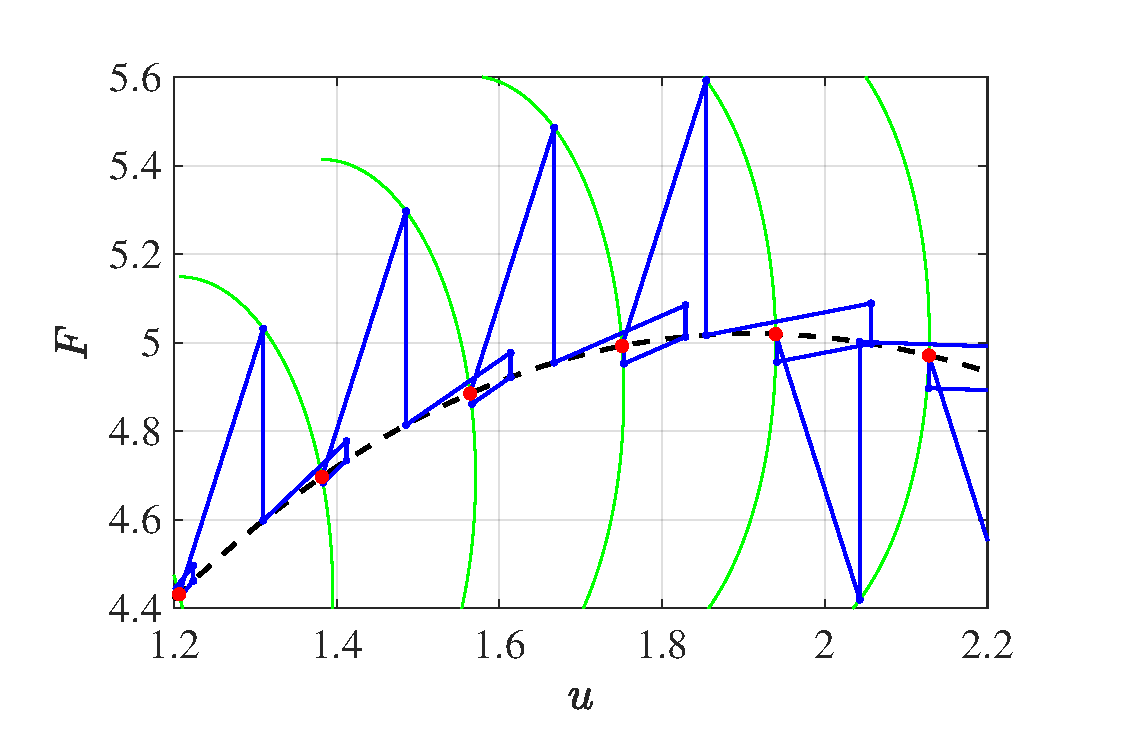
\includegraphics[width=0.7\linewidth]{homework/hw3/hw3_b0pt7_close.pdf}
    \caption{Zoomed-in version of \cref{fig:hw3_b0pt7_soln}.}
    \label{fig:hw3_b0pt7_close}
\end{figure}